\section{Editor Design}
\label{sec:editor_design}
Programming the cell is an essential part of the game. This is where the user will learn basic construct in the imperative paradigm by using them to program the initial cell and all future copies of that cell.

The editor is used by the player to design their program, that will be run during the game. To keep the overall design experience consistent, the editor will be using the same hexagonal design as the playing field. The programming will be done visually, and the hexagonal design will give the user more options for organizing their program.\\

The editor consists of two main parts, the programming grid of hexagons on the left, and individual fine tuning of elements on the right, an illustration can be seen on \autoref{fig:editor}.

\begin{figure}[ht]
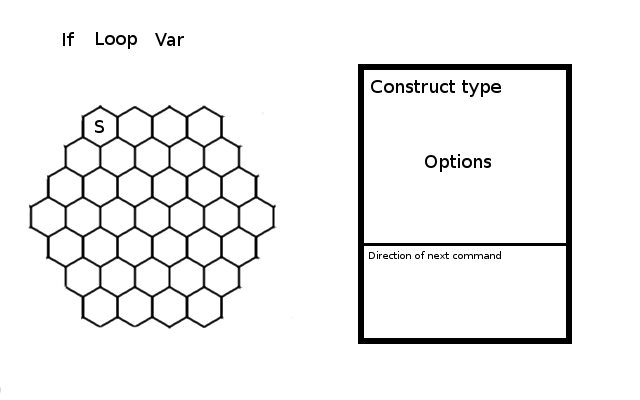
\includegraphics[width=\textwidth]{img/editor.png}
\caption{Preliminary design of the editor.}
\label{fig:editor}
\end{figure}

\subsubsection*{Programming Grid}
The programming grid makes use of a drag-and-drop interface, similar to that of the game 'Carnage Heart'.
Each programming construct, e.g. if-statements and loops, can be dragged from the top of the screen onto the hexagonal grid.
Initially this hexagonal grid only has a start point, and it is up to the player to create the program itself.
The program will be running from the start point on the grid to a user defined end point.
This end point is created by simply letting the program run outside the hexagonal grid.
By doing this, the player is essentially creating a loop, that the program will be running in during its execution.

\todo{Please check: Added from other section}It should be noted, that programming the cell should not be the cause of frustration due to the occurrence of peculiar programming-oriented errors, which the player will have to deal with.
For this reason, it is important that the interface provides the user with feedback, which gives a clear understanding of when the user has combined a string of legal or illegal programming constructs.
This can be done by implementing a basic green is correct and red is wrong color schema, that allow the user to immediately identify good code and code that includes one or more errors.
For this to work, the colors will have to be dynamic and evaluation of constructs in the program must be done on a regular basis to keep providing the player with feedback about whether the program is correct or wrong.
If the colors are not updated regularly, a construct might be flagged as red/wrong, the user corrects it, so that the construct is valid, but the construct is still flagged as red/wrong.
In general terms, it is important that the user cannot make too many construct mistakes.
Otherwise, the game is in danger of becoming a debugging game, when it should be a game about creating the most optimized and best algorithm/cell.\newline

Since the editor is using a drag-and-drop interface, adding new functionality to a program is done by dragging a construct onto the path of the current program, and define variables if needed.
Since the aim of the game is to teach programming without doing so explicitly, the variables can be define as three types/categories.
These are; numbers, entities, and directions.
The idea is that by limiting variables to three categories with meaningful names, the player will hopefully be able to easily understand what happens without prior knowledge to types in programming.
At least, this is our assumption, and if we had the time to test this, it might be possible to determine if the user would reactive positive or negative to a larger number of categories/types.

\subsubsection*{Details Panel}
The fine tuning/details panel is activated, when the player clicks on a construct, that has been placed on the hexagonal grid.
If it is deselected the fine tuning panel disappears until another construct is selected.
The panel will show different information depending on what kind of construct the player has clicked on.
For example, one of the options available for the if-statement includes a list of variables, that the if-statement can compare to generate a scenario where the variable can be in a true or false state, making the if work.
A move construct, however, will only include the option to define in which direction the cell will move.
The bottom part of the fine tuning panel is used by the player to choose, which tile on the hexagonal grid the program should be going to next.
This can be used to structure the program or make it possible for the player to customize the grid to their liking.
However, it also allows the user the freedom to create infinite loops.
Since it is NP-hard to find infinite loops in a program, we can not check the program for infinite loops for the user.
Therefore, we leave it up to the user to find these loops. 

\subsection{Design Decisions}
Several design decisions have been made for the editor.
Firstly, it was clear from the beginning, that the editor should utilize some kind of visual interface for programming, since this was used in the programming games, 'Carnage Heart' and 'Kodu Game Lab'.
If the player had to write code explicitly, it would be very clear, that the game is trying to teach programming, which goes against our goals for this project.\newline

When it was decided that the programming interface would be visual, the idea of a grid quickly became the preferred method.
As described in \autoref{sec:teachProgWithGames}, the game 'Carnage Heart' make use of a similar grid interface for programming.
It was chosen, that the editor should keep the look and feel from the game board, and thus it also makes use of a hexagonal grid.
The hexagonal grid has some features, which made preferable to a standard square grid.
The hexagonal grid makes it possible for the player to have more options as to how the program is structured.
It also makes it possible for the two branches of an if statement or a loop to be next to each other rather than on different sides of a square.\newline

The details panel was more difficult to design, since the options available are different for every construct.
Since it was decided, that the editor should utilize a visual programming interface with drag-and-drop, the player would need to be able to set some amount of variables for the program to be functional enough, such as a condition in an if-statement.
The details panel was chosen\todo{Maybe include: over what alternative}, because it removes the need to exit out of the details panel to be able to switch to the details of another construct on the grid, if the details were to pop up over the hexagonal grid.
The details panel on the right side of the hexagonal grid effectively eliminates a number of steps, with the purpose to make the game quicker and less frustrating to use.
